\renewcommand{\theequation}{\theenumi}
\begin{enumerate}[label=\thesection.\arabic*.,ref=\thesection.\theenumi]
\numberwithin{equation}{enumi}

\item $\vec{x}=\myvec{x\\y}$ is the solution, Then for every value of x , there is corresponding value of y. 
Let $\vec{A_1}=\myvec{0\\a_1}$ and $\vec{B_1}=\myvec{1\\b_1}$ be the two solutions of equation \ref{eq:pointonline1}.Then
\begin{align}
 \myvec{4&3}\myvec{0\\a_1}=12
 \implies a_1=4
 \\
 \myvec{4&3}\myvec{1\\b_1}=12
 \implies b_1=\frac{8}{3}
\end{align}
So $\myvec{0\\4}$ and $\myvec{1\\\frac{8}{3}}$ are the two solutions of \ref{eq:pointonline1}

\item 
Let $\vec{A_2}=\myvec{0\\a_2}$ and $\vec{B_2}=\myvec{1\\b_2}$ be the two solutions of equation \ref{eq:pointonline2}.Then
\begin{align}
 \myvec{2&5}\myvec{0\\a_2}=0
 \implies a_2=0
 \\
 \myvec{2&5}\myvec{1\\b_2}=0
 \implies b_2=\frac{-2}{5}
\end{align}

So $\myvec{0\\0}$ and $\myvec{1\\\frac{-2}{5}}$ are the two solutions of \ref{eq:pointonline2}
\item 
Let $\vec{A_3}=\myvec{0\\a_3}$ and $\vec{B3}=\myvec{1\\b_3}$ be the two solutions of equation \ref{eq:pointonline3}.Then
\begin{align}
 \myvec{0&3}\myvec{0\\a_3}=4
 \implies a_3=\frac{4}{3}
 \\
 \myvec{0&3}\myvec{1\\b_3}=4
 \implies b_3=\frac{4}{3}
\end{align}
So $\myvec{0\\\frac{4}{3}}$ and $\myvec{1\\\frac{4}{3}}$ are the two solutions of \ref{eq:pointonline3}

The following Python code generates Fig. \ref{fig:point_on_line} showing a graph of lines representing the equations \ref{eq:pointonline2} \ref{eq:pointonline1}and \ref{eq:pointonline3}. It can be verified that the solutions of above equations lie on the lines
%
\begin{lstlisting}
codes/line/pointonline/pointonline.py
\end{lstlisting}
\begin{figure}[!ht]
\centering
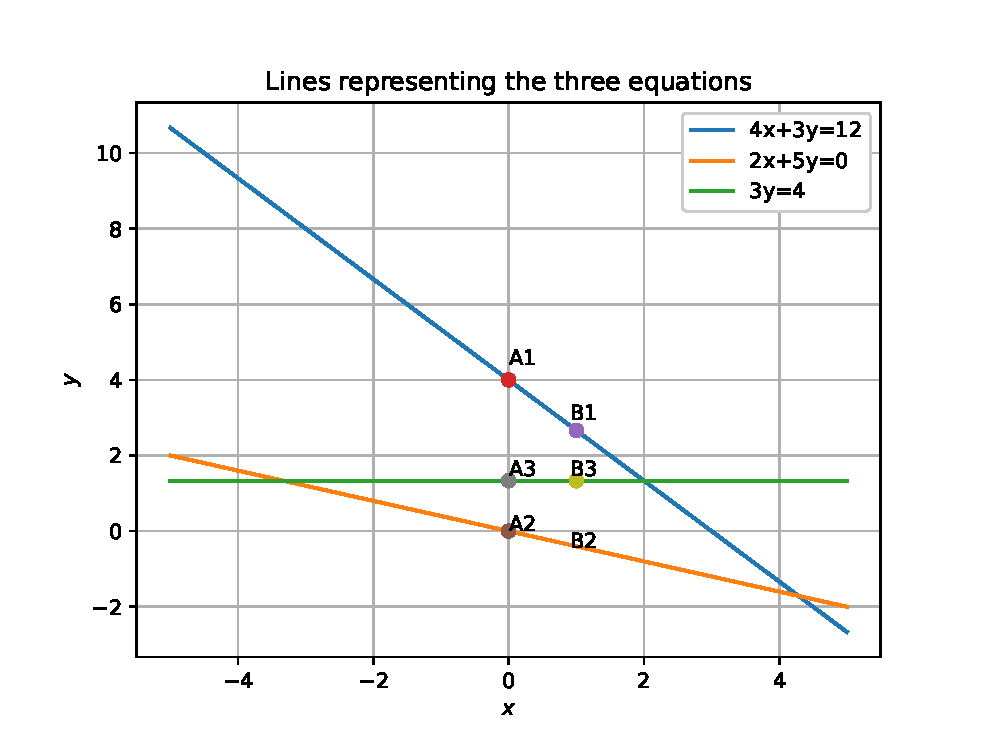
\includegraphics[width=\columnwidth]{./codes/line/pointonline/pyfigs/pointonline.eps}
\caption{Lines representing equations}
\label{fig:point_on_line}
\end{figure}
\end{enumerate}
